\chapter{ANALISIS}
\section{System Definition}
\begin{figure}[h]
	\centering
	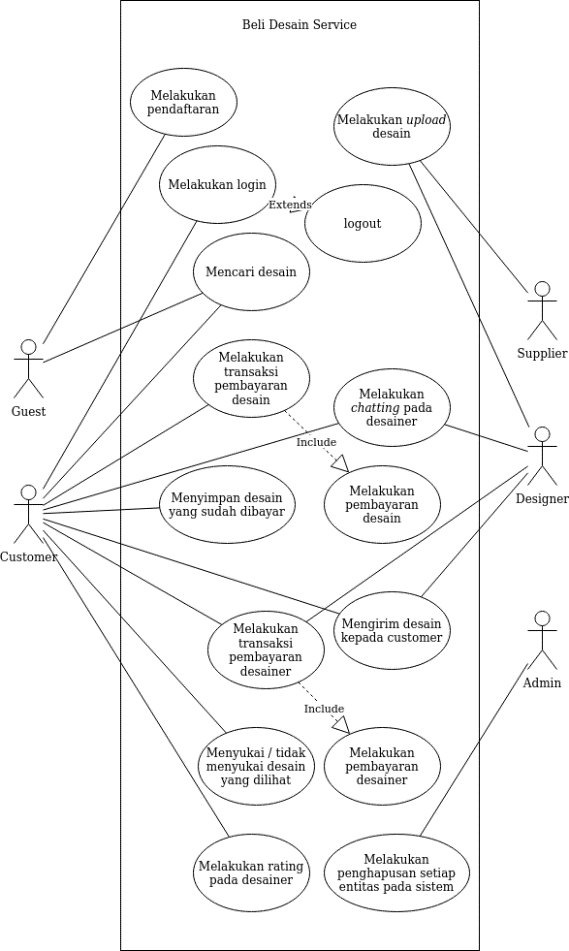
\includegraphics{usecase}
	\caption{Use Case Diagram Sistem Belidesain}
\end{figure}

\section{Identifikasi Permasalahan}
Berdasarkan latar belakang yang telah ditulis, terdapat beberapa identifikasi masalah yang dapat disimpulkan yaitu sebagai berikut:
\begin{enumerate}
	\item Penjualan desain pada platform e-commerce jarang ditemui.
	\item Penyebaran informasi pameran desain yang belum meluas.
	\item Pencarian jasa desainer panggilan masih jarang ditemui.
\end{enumerate}

\section{Identifikasi Kebutuhan Pengguna}
Semakin berkembangnya teknologi, gaya hidup masyarakat ikut serta berubah. Di era yang sekarang, gaya hidup yang diikuti masyarakat adalah gaya hidup modern. Kebutuhan masyarakat pun tidak jauh dari hal yang berkaitan dengan desain, seperti pakaian, barang perabot, dan lain-lain. Ketika akan membeli pasti mencari desain yang cocok dengan selera dan kebutuhan. Tidak jarang desain yang dicari tidak sesuai dengan selera.
\par Dalam memenuhi kebutuhan masyarakat akan desain yang sesuai selera, sistem yang kami buat dapat menjadi jawabannya. Sistem berisikan informasi terkait penjualan desain. Pelanggan dapat melihat-lihat terlebih dahulu terkait desain yang dicari. Apabila sudah menemukan yang sesuai, pelanggan dapat melakukan transaksi. Jika desain yang dicari tidak ada yang cocok, pelanggan dapat meminta desainer untuk membuatkan desain yang diinginkan. Semua hasil transaksi dan yang lainnya akan terekam dalam sistem database kami. 
